\chapter{Denial of Service}

\section{Basic Model Design}

In the previous section, we discussed a basic model where the system had N queues, arrival rate was $\lambda_i$, service rate was $\mu_i$, utilization was $\rho_i$ and we described the probability of the system containing $a_i$ number of antivirus, $v_i$ number of virus and $d_i$ number of antivirus and virus interactions. The probability was given by :

$$\mathbf{P_{((a_1,v_1,d_1),.....,(a_N,v_N,d_N))} =      \prod_{i=1}^{N} (1-\rho_i){{\rho_i}^{a_i+v_i+2d_i}} }$$

Now extending this analogy, suppose $a_i$ denotes the number of normal request packets entering the system, $v_i$ denotes the number of malicious packets entering the system. If there is no interaction between these packets, then $d_i$ is 0 and the expected result will be:

$$\mathbf{P_{((a_1,v_1),.....,(a_N,v_N))} = \prod_{i=1}^{N} (1-\rho_i){{\rho_i}^{a_i+v_i}} }$$

$(a_i,v_i)$ denotes the queue i having $a_i$ number of normal packets and $v_i$ number of malicious packets. So for N nodes the probability to be in a particular state $\mathbf{n(t)}$ $=((a_1,v_1),.....(a_N,v_N))$ is given by the product form solution of $$\prod_{i=1}^{N} (1-\rho_i){{\rho_i}^{a_i+v_i}} $$

\section{Single Node Network:} 

If we have single node in the network and we model that node as an M/M/1 queue with infinite size, Then the probability of server  having $a$ normal packets and $v$ malicious packets is given by: 

$$\mathbf{P_{(a,v)} =(1-\rho){{\rho}^{a+v}} }$$

where a denotes the number of normal packets in the node where as v denotes the number of malicious packets in the node.

\subsection{Numerical Results}

We try to study the above described result by varying the parameters. 

\paragraph{Varying $\rho :$}

For a single server system, $\rho$ is a measure of utilization as well as traffic intensity of a network. For a stable system $\rho$ should be between 0 and 1. If we vary $\rho$ to find the maximum probability of reaching a given $a$ and $v$, we know that maximum probability occurs when:
\begin{center}
$\frac{\partial P}{\partial \rho} = 0 \Rightarrow\quad \rho= \frac{a+v}{a+v+1}$ 
\end{center}

Initially when $\rho$ is near to 0, i.e. when mean arrival time is quite large compared to mean service time, then the traffic intensity is very low i.e as soon as the packet arrives it is served, hence probability to reach a certain state $a,v$ is also very low. Now as the system become more traffic intense, mean arrival time decreases and the mean service time increases, and the probability to reach a certain state $a,v$ also increases upto a certain limit. Now as $\rho$ tends to 1, i.e the system become most traffic intense, then the probability to reach that state $a,v$ again goes to 0. 

\begin{figure}[H]
		\centering
		\resizebox{1\linewidth}{!}{\includegraphics{figa}}
		\caption{{Probability of reaching a,v by varying traffic intensity }}
		\label{fig:figa}
\end{figure}

From the above graph, we see that the maximum probability to reach a certain state $a,v$ for all the three cases occurs when $\rho$ is near to 1. Our theoretical result also points that maximum probability is at $\frac{a+v}{a+v+1}$ which is quite nearer to 1. Apart from that, we observe that if the number of malicious packets increase, probability to reach $a,v$ goes down further. Thus, as the value of $v$ increases, maximum probability occurs more nearer to 1, but the maximum probability goes on decreasing. With less number of packets, we have more probability to reach certain state, compared to more number of packets. All the three cases have similar behavior when $\rho$ is less than 0.3 and very very close to 1. So, to study the behavior of a node, we should mainly focus on the traffic intensity between 0.3 and 1;   

\paragraph{Varying v:} If we vary number of malicious packets keeping traffic intensity and number of normal packets fixed:

\begin{figure}[H]
		\centering
		\resizebox{0.8\linewidth}{!}{\includegraphics{figb}}
		\caption{{Probability of reaching a,v by taking a=1 and varying v}}
		\label{fig:figb}
\end{figure}


As the number of malicious packets increase, the probability to be on a certain state $a,v$ goes on decreasing. We assume that our system has only one normal packet. We know that low values of $\rho$ indicate that mean service time is faster than mean arrival time. So, as the number of malicious packets increase, probability to reach certain state $a,v$ goes to 0 quickly for low traffic intense systems. For a given malicious packets, if we draw a vertical line in our graph, we see that for $\rho=0.5$ we get the maximum probability to reach a certain state $a,v$. If we increase the number of normal packets, probability to reach a particular state converges to 0 more rapidly. 

\pagebreak

\paragraph{$\mathbf{n^{th}}$ packet gets dropped:}
 Now let us assume that the $n^{th}$ packet received by system is dropped after the start i.e denial of service occurs for the $n^{th}$ packet. Then, we can say that when the $n^{th}$ packet arrives the system contains either $(0,n-1)$ or $(1,n-2)$ or $......$ or $(n-1,0)$ number of normal and malicious packets. Probability that the service is denied is given by :

$$P_{denial} =(1-\rho){{\rho}^{0+n-1}} + (1-\rho){{\rho}^{1+n-2}} + .......  + (1-\rho){{\rho}^{n-1+0}}$$
$$\Rightarrow P_{denial}=n(1-\rho){{\rho}^{n-1}} $$ 

\subparagraph{Varying $\rho$:} If we vary $\rho$, taking n fixed  we get:

\begin{center}
$\frac{\partial P_{denial}}{\partial \rho} = 0 \Rightarrow\quad \rho= \frac{n-1}{n}$ 
\end{center}

\begin{figure}[H]
		\centering
		\resizebox{1\linewidth}{!}{\includegraphics{figc}}
		\caption{{Probability of packet loss Varying rho for different n}}
		\label{fig:figc}
\end{figure}


For a fixed value of n, the value of $\rho$ for which we get maximum probability of $n^{th}$ packet being dropped is given by  $\frac{n-1}{n}$. As the value of n increases, more and more, the $\rho$ value to have maximum probability of the $n^{th}$ packet being dropped tends to 1, while the probability in itself goes on decreasing. This is because if we substitute $\rho$ in the equation for which maximum probability occurs, we get the maximum probability as ${(\frac{n-1}{n})}^{n-1}$ and as n increases the value become smaller and smaller. For, low values of traffic intensity, service time is faster than the arrival time, so the probability of packet being dropped is very less. As the value of traffic intensity increases, the probability to drop packets increases slowly. Once the probability reaches maximum, it decreases very rapidly. Thus, for lower values of traffic intensity change in probability is lower compared to higher values of traffic intensity. 
\subparagraph{Varying $n$:}If we vary $n$ taking fixed $\rho:$

\begin{figure}[H]
		\centering
		\resizebox{0.9\linewidth}{!}{\includegraphics{figd}}
		\caption{{Probability of packet drop by varying n taking different rho}}
		\label{fig:figd}
\end{figure}

If we take smaller values of $\rho$, graph is mainly distorted and since we have shown that our main point of concentration should be when $\rho$ varies from 0.4 to 1. so we take five different values of $\rho$ and try to vary n. If $\rho$ is small then for very small value of n, we get the maximum probability of packet being lost. As the value of $\rho$ increases, we get a little larger value of n, for the maximum probability of a packet to be lost while the probability in itself goes on decreasing. If we draw a vertical line after n=8 packets, we see that higher the value of $\rho$, higher is the probability of a packet being lost. This result holds in with the fact that higher value of $\rho$ indicate that mean arrival time is less and mean service time is more and hence probability of packet being dropped is more. If we want to find the probability of a packet being lost for smaller values of n, say 2, then we see that the probability of packet being lost for lower values of $\rho$ is much more than that of higher value of $\rho$. So, we conclude that if for a smaller n, the packets are dropped, then the probability to drop packets for smaller values of $\rho$ is more than larger values of $\rho$ and for larger n, larger values of $\rho$ are more probable to drop packets.

\subparagraph{Varying $n$ and $\rho$:} If we vary n and $\rho$ together we observe that for smaller values of n, for a very small $\rho$ we get very high probability of the packet being dropped compared to larger values of $\rho$ while for values of n greater than 5, we have high probability of packet being dropped for larger values of $\rho.$  

\begin{figure}[H]
		\centering
		\resizebox{1\linewidth}{!}{\includegraphics{fige}}
		\caption{{Probability of packet being dropped varying n and rho}}
		\label{fig:fige}
\end{figure}

Thus, the probability of packet being dropped is similar to denying service to that packet and we have studied the probability of packet being dropped by varying $\rho$ and $n$ and both of them together.

\pagebreak

\section{Network Simulations}

For practical purposes, we present network simulations of Denial of Service Attacks. We basically focus on two fields: UDP attack over UDP client and UDP attack over TCP client. We do not consider TCP attacker because TCP protocol is for reliable transmission of the packets and an attacker's only aim is to prevent normal packets from reaching the destination not to ensure the delivery of attack packets.

\subsection{UDP Attacker over UDP client}

Here we study the system parameters in both presence and absence of attacker. We take a simple topology as described below:

\begin{figure}[!htb]
		\centering
		\resizebox{1\linewidth}{!}{\includegraphics{basic}}
		\caption{{Absence of Attacker Configuration}}
		\label{fig:figf}
\end{figure}

\begin{figure}[!htb]
		\centering
		\resizebox{1\linewidth}{!}{\includegraphics{basic1}}
		\caption{{Presence of Attacker Configuration}}
		\label{fig:figg}
\end{figure}

\subsubsection{Description of our Topology} 

\begin{itemize}

\item \textbf{Client Packets:} Packets are generated at the client side at an exponenial rate i.e the packets follow exponential arrival rate at the server and the packets have varying length and the lengths are simulated by exponential distribution. Varying packet lengths produces exponential service rate.

\item \textbf{Attacker Packets:} The attacker packets also follow exponential service rate but have uniform packet size and hence uniform service rate.

\item \textbf{Link Description:} Each links have 100 ms propagation delay and 0.5Mbps link speed in a fixed Bandwidth case i.e Each links are of same length and Each link provides equal service.

\item \textbf{Queue Description:} Our Queuing model follows M/D/1/K model i.e the arrival rate is exponential, service rate is uniform, single server and queue size is k. We fix our Queuing size to be 15.

\item \textbf{Protocol Description:} Our client and attacker on the left hand side (as shown in figure ~\ref{fig:figg}) both connects with User Datagram Protocol with both the clients on the right hand side. Each packet has a certain random probability which decides the receiver of the packet.

\item \textbf{Simulation Time:} We simulate the entire duration for 100 secs. For the first 10 secs normal packet generation takes place. After 10 secs the attacker starts working. At t=40 sec, the attacker stops working and at t=60 sec it starts again. At t=90 sec the attacker finishes itself and finally at t=100 sec normal packet generation also stops.

\end{itemize}

\subsubsection{Network Simulation Code}
\lstinputlisting[caption=\texttt{NS2}  Code which simulates the network, label=lst:q1, language=C]{../Codes/udp_udp/Simulations/attack3.tcl}

\subsubsection{Experimental Analysis and Results:}
\medskip

For simulation purpose we run 100 simulations to produce our results. We basically study five things: Expected Throughput, Expected probability of packet being dropped, Expected number of packets being dropped, Expected size of queue, Expected waiting time in a queue. The parameters, we vary to study these parameters are: time, Arrival Rate, Service Rate and Bandwidth. The parameters are studied in both presence and absence of attacker. 
  
\subsubsection*{Fixed Arrival Rate, Service Rate and Bandwidth:}

\begin{figure}[!htb]
	\centering
	\subfloat[Number of packets dropped]{\includegraphics[width=7cm]{../Codes/udp/Simulations/Results/pacdrop}}%
	\qquad
	\subfloat[Probability of packets dropped ]{\includegraphics[width=7cm]{../Codes/udp/Simulations/Results/prdrop}}%
	\caption{{Number of Packets and probability of packet being dropped in absence of Attacker Configuration}}
	\label{fig:figab}
\end{figure}

\begin{figure}[!htb]
	\centering
	\subfloat[Number of packets dropped]{\includegraphics[width=7cm]{../Codes/udp_udp/Simulations/Results/pacdrop}}%
	\qquad
	\subfloat[Probability of packets dropped ]{\includegraphics[width=7cm]{../Codes/udp_udp/Simulations/Results/prdrop}}%
	\caption{{Number of Packets and probability of packets dropped in presence of Attacker Configuration}}
	\label{fig:figac}
\end{figure}

As attack starts at time t=10 sec, the number of packets being dropped starts increasing. As we switch off the attack, the packets dropped almost tends to 0 which is similar to the case when there is no attacker and the number of packets being dropped is almost 0. Similar situation exists for the probability of packet being dropped. 

\pagebreak

\begin{figure}[!htb]
	\centering
	\subfloat[Presence of Attacker]{\includegraphics[width=7cm]{../Codes/udp_udp/Simulations/Results/queuelen}}%
	\qquad
	\subfloat[Absence of Attacker]{\includegraphics[width=7cm]{../Codes/udp/Simulations/Results/queuelen}}%
	\caption{{Expected Queue length in terms of packets}}
	\label{fig:figad}
\end{figure}

During the presence of attack, large number of packets are generated and hence the queue size is almost full. When we switch off the attack, queue size tends to almost 0.

\begin{figure}[!htb]
	\centering
	\subfloat[Presence of Attacker]{\includegraphics[width=7cm]{../Codes/udp_udp/Simulations/Results/waiting}}%
	\qquad
	\subfloat[Absence of Attacker ]{\includegraphics[width=7cm]{../Codes/udp/Simulations/Results/waiting}}%
	\caption{{Expected waiting time in a queue}}
	\label{fig:figae}
\end{figure}

We know that waiting time is proportional to the queue size. More the queue size, more is the waiting time. In absence of attacker both queue sizes and waiting time is very low. Waiting time is almost 10 times in presence of attacker compared to the absence of attacker. 

\pagebreak

\begin{figure}[!htb]
	\centering
	\subfloat[Presence of Attacker]{\includegraphics[width=7cm]{../Codes/udp_udp/Simulations/Results/systhroughput}}%
	\qquad
	\subfloat[Absence of Attacker ]{\includegraphics[width=7cm]{../Codes/udp/Simulations/Results/systhroughput}}%
	\caption{{Expected Throughput vs Time}}
	\label{fig:figaf}
\end{figure}

If number of packets flowing through the system increases, system throughput increases due to more and more utilisation. Higher the link utilisation, higher the number of packets dropped. System throughput is almost 1.5 times in presence of attacker compared to the absence of attacker.   

\subsubsection*{Varying Arrival Rate, fixed Service Rate and Bandwidth:}

\begin{figure}[H]
		\centering
		\resizebox{0.7\linewidth}{!}{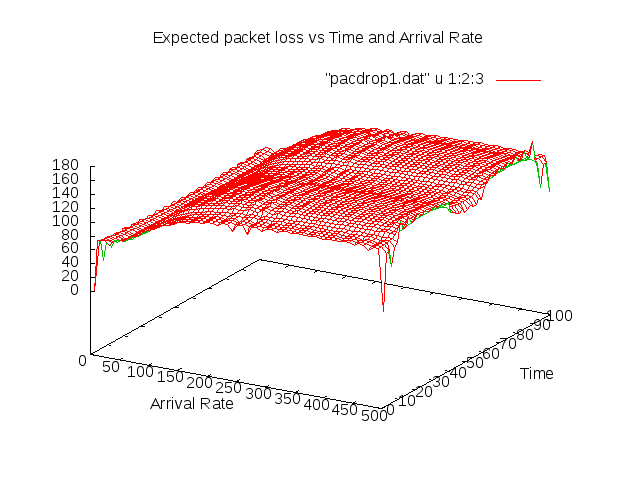
\includegraphics{../Codes/udp_udp/Simulations/Results/pacdrop1}}
		\caption{{Expected number of packets dropped in presence of Attacker Configuration varying Arrival Rate}}
		\label{fig:figba}
\end{figure}

\pagebreak

In absence of attacker, expected number of packets dropped is less than 1 but in presence of attacker, as the arrival rate increases, number of packets dropped goes on increasing. As the time increases, expected number of packets dropped also goes on increasing. When we switch off the attacker between 40 and 60 secs, packets dropped decreases so we find a buldge in our graph. Expected probability of packets being lost behave in a similar manner.

\begin{figure}[H]
		\centering
		\resizebox{0.7\linewidth}{!}{\includegraphics{../Codes/udp/Simulations/Results/prdrop1}}
		\caption{{Expected probability of packets dropped in absence of Attacker Configuration varying Arrival Rate}}
		\label{fig:figbb}
\end{figure}

\begin{figure}[H]
		\centering
		\resizebox{0.5\linewidth}{!}{\includegraphics{../Codes/udp_udp/Simulations/Results/prdrop1}}
		\caption{{Expected probability of packets dropped in presence of Attacker Configuration varying Arrival Rate}}
		\label{fig:figbc}
\end{figure}

\pagebreak

\begin{figure}[H]
		\centering
		\resizebox{0.6\linewidth}{!}{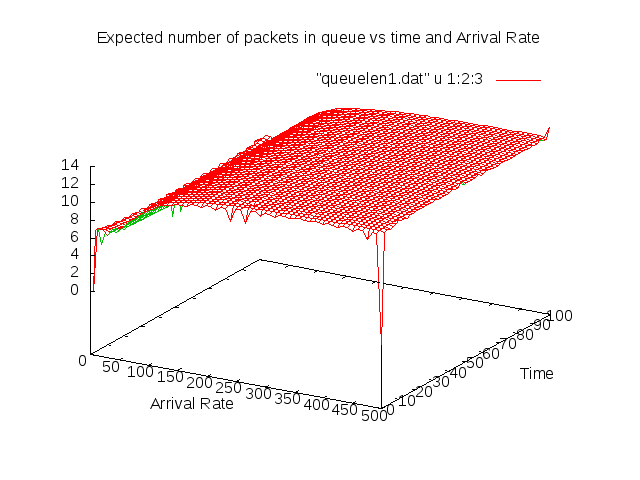
\includegraphics{../Codes/udp_udp/Simulations/Results/queuelen1}}
		\caption{{Expected number of packets in queue in presence of Attacker Configuration varying Arrival Rate}}
		\label{fig:figbd}
\end{figure}

\begin{figure}[H]
		\centering
		\resizebox{0.6\linewidth}{!}{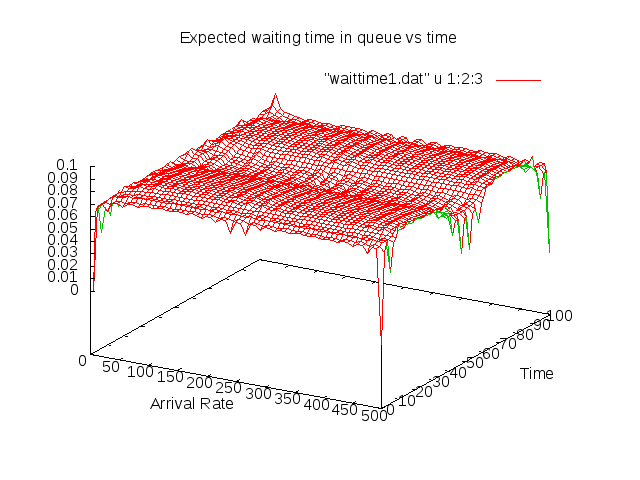
\includegraphics{../Codes/udp_udp/Simulations/Results/waiting1}}
		\caption{{Expected waiting time in presence of Attacker Configuration varying Arrival Rate}}
		\label{fig:figbe}
\end{figure}

As the arrival rate increases, queue length increases because the number of packets increases in the system. Hence the waiting time also goes on increasing. Queue length is almost full for large value of arrival rate. Without the presence of attacker, queue length is uniform through out time.

\pagebreak

\begin{figure}[H]
		\centering
		\resizebox{0.6\linewidth}{!}{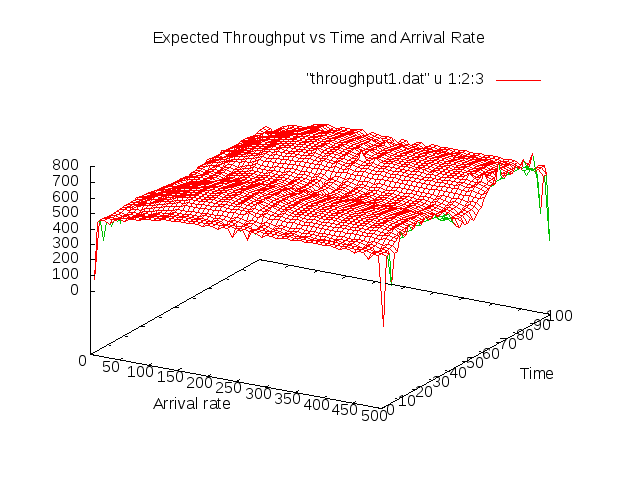
\includegraphics{../Codes/udp_udp/Simulations/Results/systhroughput1}}
		\caption{{Expected Throughput in presence of Attacker Configuration varying Arrival Rate}}
		\label{fig:figbf}
\end{figure}

Increase in arrival rate results in increase of number of packets which in result increases the link utilisation.
 
\subsubsection*{Varying Service Rate, fixed Arrival Rate and Bandwidth:}

\begin{figure}[H]
		\centering
		\resizebox{0.7\linewidth}{!}{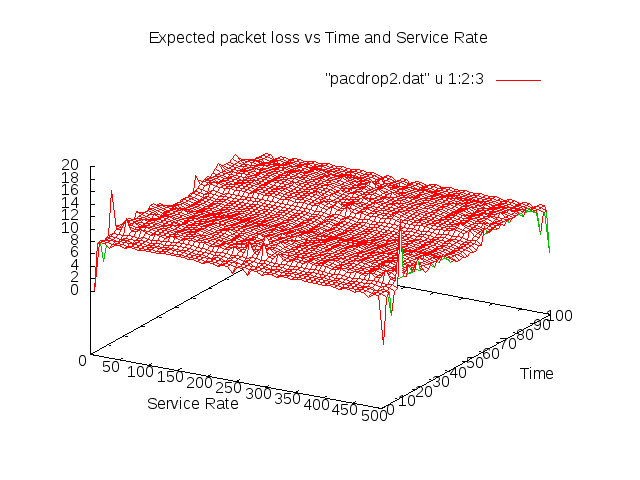
\includegraphics{../Codes/udp_udp/Simulations/Results/pacdrop2}}
		\caption{{Expected number of packets dropped in presence of Attacker Configuration varying Service Rate}}
		\label{fig:figca}
\end{figure}

\pagebreak

For low values of service rate, expected number of packets dropped is very large. As the value of service rate increases, as soon as the packet arrives, it is served hence queue is almost empty and packet loss goes on decreasing and it almost goes to 0 for large value of service rate. Similar behaviour occurs for expected probability of packet being dropped. 

\begin{figure}[H]
		\centering
		\resizebox{0.7\linewidth}{!}{\includegraphics{../Codes/udp/Simulations/Results/prdrop2}}
		\caption{{Expected probability of packets dropped in absence of Attacker Configuration varying Service Rate}}
		\label{fig:figcb}
\end{figure}

\begin{figure}[H]
		\centering
		\resizebox{0.5\linewidth}{!}{\includegraphics{../Codes/udp_udp/Simulations/Results/prdrop2}}
		\caption{{Expected probability of packets dropped in presence of Attacker Configuration varying Service Rate}}
		\label{fig:figcc}
\end{figure}

\pagebreak

\begin{figure}[H]
		\centering
		\resizebox{0.6\linewidth}{!}{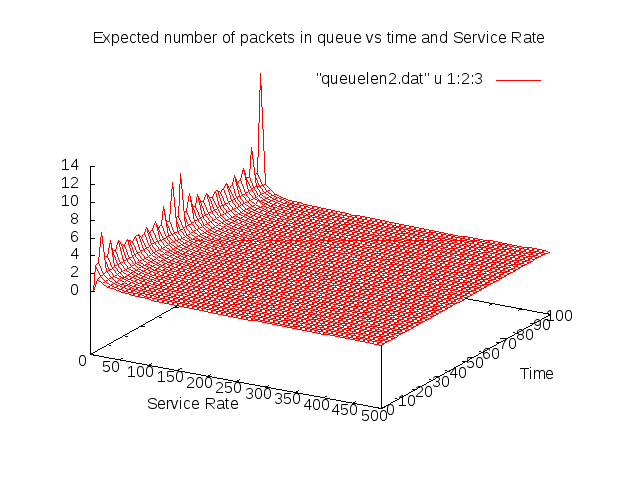
\includegraphics{../Codes/udp_udp/Simulations/Results/queuelen2}}
		\caption{{Expected number of packets in queue in presence of Attacker Configuration varying Service Rate}}
		\label{fig:figcd}
\end{figure}

\begin{figure}[H]
		\centering
		\resizebox{0.6\linewidth}{!}{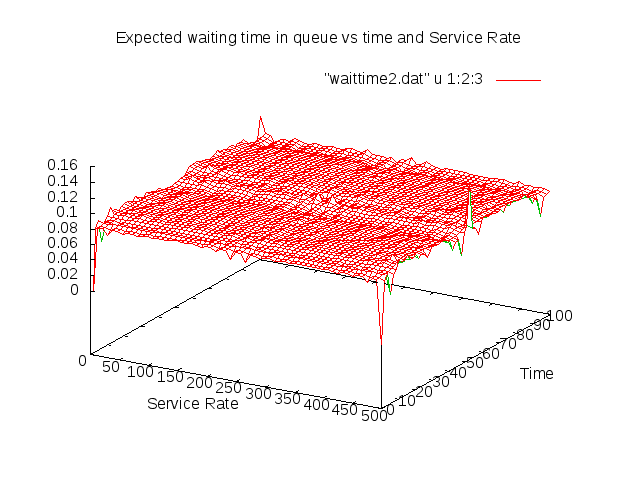
\includegraphics{../Codes/udp_udp/Simulations/Results/waiting2}}
		\caption{{Expected waiting time in presence of Attacker Configuration varying Service Rate}}
		\label{fig:figce}
\end{figure}

As the service rate increases, queue length decreases because the number of packets decreases in the system because the packets are served very quickly. Hence the waiting time also goes on decreasing. Queue length is almost full for snmall values of service rate. Without the presence of attacker, queue length is uniform through out time. Between 40.0 and 60.0 secs, when we stop the attacker queue length further goes down for small values of survival rate. For larger values of service rate, queue length is uniform through out time and hence it is almost 0.

\begin{figure}[H]
		\centering
		\resizebox{0.6\linewidth}{!}{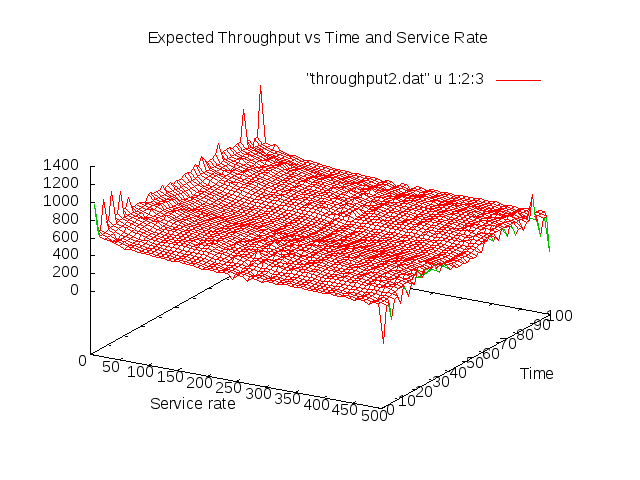
\includegraphics{../Codes/udp_udp/Simulations/Results/systhroughput2}}
		\caption{{Expected Throughput in presence of Attacker Configuration varying Service Rate}}
		\label{fig:figcf}
\end{figure}

Increase in service rate results in decrease of number of packets which in result decreases the link utilisation.
 
\subsubsection*{Varying Bandwidth, fixed Arrival Rate and Service Rate:}

\begin{figure}[H]
		\centering
		\resizebox{0.5\linewidth}{!}{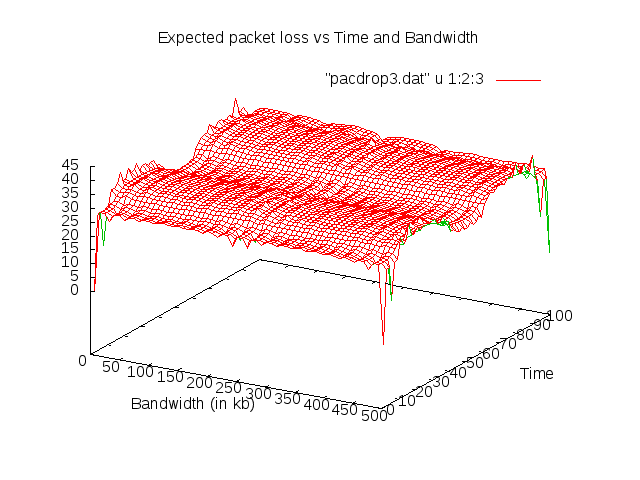
\includegraphics{../Codes/udp_udp/Simulations/Results/pacdrop3}}
		\caption{{Expected number of packets dropped in presence of Attacker Configuration varying bandwidth}}
		\label{fig:figdb}
\end{figure}

\pagebreak

For low values of Bandwidth, expected number of packets dropped is very large. As the value of Bandwidth increases, packets are served quickly, hence queue is almost empty and packet loss goes on decreasing and it almost goes to 0 for large value of Bandwidth. Similar behaviour occurs for expected probability of packet being dropped. 

\begin{figure}[H]
		\centering
		\resizebox{0.6\linewidth}{!}{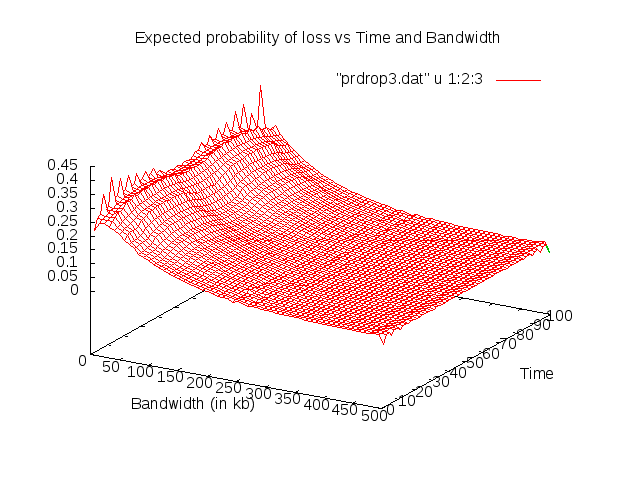
\includegraphics{../Codes/udp_udp/Simulations/Results/prdrop3}}
		\caption{{Expected probability of packets dropped in presence of Attacker Configuration varying bandwidth}}
		\label{fig:figdc}
\end{figure}

\begin{figure}[H]
		\centering
		\resizebox{0.7\linewidth}{!}{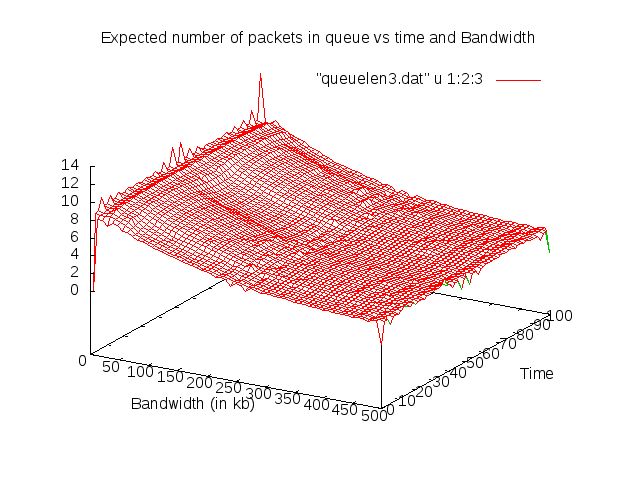
\includegraphics{../Codes/udp_udp/Simulations/Results/queuelen3}}
		\caption{{Expected number of packets in queue in presence of Attacker Configuration varying bandwidth}}
		\label{fig:figdd}
\end{figure}

\pagebreak

\begin{figure}[H]
		\centering
		\resizebox{0.6\linewidth}{!}{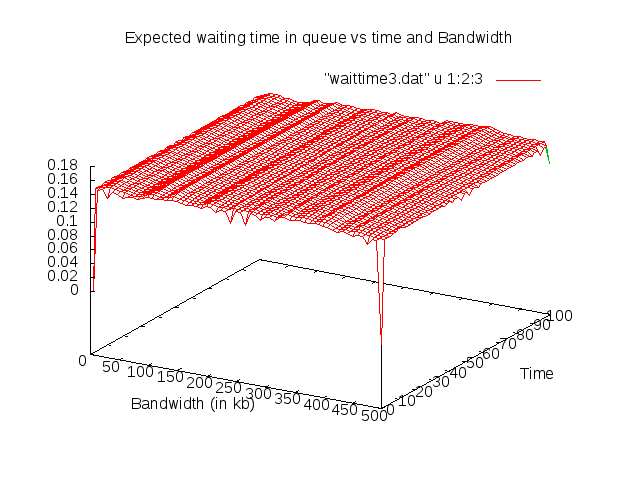
\includegraphics{../Codes/udp_udp/Simulations/Results/waiting3}}
		\caption{{Expected waiting time in presence of Attacker Configuration varying bandwidth}}
		\label{fig:figde}
\end{figure}

\begin{figure}[H]
		\centering
		\resizebox{0.6\linewidth}{!}{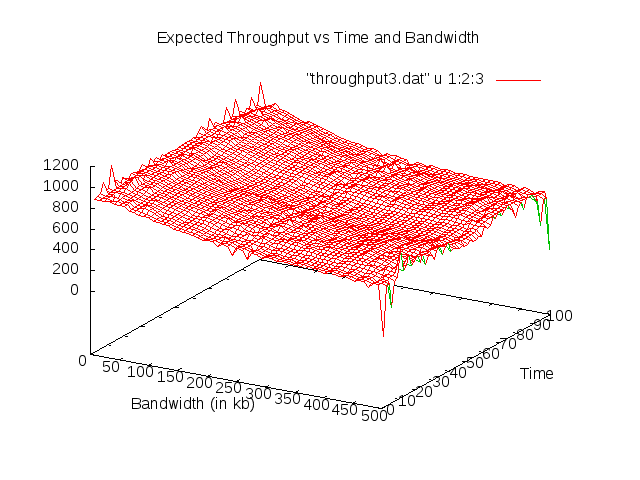
\includegraphics{../Codes/udp_udp/Simulations/Results/systhroughput3}}
		\caption{{Expected Throughput in presence of Attacker Configuration varying Bandwidth}}
		\label{fig:figdf}
\end{figure}

As the Bandwidth increases, queue length decreases because the number of packets decreases in the system because the packets are served very quickly. Hence the waiting time also goes on decreasing. Queue length is almost full for small values of Bandwidth since packets are served very slowly. Increase in Bandwidth results in decrease of number of packets which in result decreases the link utilisation. 

\pagebreak

\subsection{UDP Attacker over TCP client}

We take the same model as described in figure ~\ref{fig:figg}. But instead of UDP client we take a TCP client on the left side and try to study system performance. Transmission Control Protocol provides better flow control, congestion control and error detection mechanism compared to UDP. Once the packets are lost we have no control over the packet in UDP but in TCP due to retransmission 
system study becomes more complicated to study. 

\subsubsection{Description of our Topology} 

\begin{itemize}

\item \textbf{Client Packets:} Packets are generated at the client side at an exponenial rate i.e the packets follow exponential arrival rate at the server. Since our client is a TCP connection, packets are generated at the multiple of 2 unless packet drop occurs in which case generation takes place linearly.  

\item \textbf{Attacker Packets:} The attacker packets also follow exponential service rate but have uniform packet size and hence uniform service rate.

\item \textbf{Link Description:} Each links have 100 ms propagation delay and 0.5Mbps link speed in a fixed Bandwidth case i.e Each links are of same length and Each link provides equal service.

\item \textbf{Queue Description:} Our Queuing model follows M/D/1/K model i.e the arrival rate is exponential, service rate is uniform, single server and queue size is k. We fix our Queuing size to be 15.

\item \textbf{Protocol Description:} Our client and attacker on the left hand side (as shown in figure ~\ref{fig:figg}) both connects with Transmission Control Protocol with both the clients on the right hand side. Each packet has a certain random probability which decides the receiver of the packet.

\item \textbf{Simulation Time:} We simulate the entire duration for 100 secs. For the first 10 secs normal packet generation takes place. After 10 secs the attacker starts working. At t=40 sec, the attacker stops working and at t=60 sec it starts again. At t=90 sec the attacker finishes itself and finally at t=100 sec normal packet generation also stops.

\end{itemize}

\subsubsection{Experimental Analysis and Results:}
\medskip

For simulation purpose we run 100 simulations to produce our results. We basically study five things: Expected Throughput, Expected probability of packet being dropped, Expected number of packets being dropped, Expected size of queue, Expected waiting time in a queue. The parameters, we vary to study these parameters are: time, Arrival Rate, Service Rate and Bandwidth. The parameters are studied in both presence and absence of attacker. 
  
\subsubsection*{Fixed Arrival Rate, Service Rate and Bandwidth:}

\begin{figure}[!htb]
	\centering
	\subfloat[Number of packets dropped]{\includegraphics[width=7cm]{../Codes/tcp_udp/Simulations/Results/pacdrop}}%
	\qquad
	\subfloat[Probability of packets dropped ]{\includegraphics[width=7cm]{../Codes/tcp_udp/Simulations/Results/prdrop}}%
	\caption{{Number of Packets and probability of packets dropped in presence of Attacker Configuration}}
	\label{fig:figac1}
\end{figure}

As attack starts at time t=10 sec, expected number of packets being dropped starts increasing. As we switch off the attack, the packets dropped almost tends to 0 which is similar to the case when there is no attacker and the number of packets being dropped is almost 0. Similar situation exists for the expected probability of packet being dropped. The expected number of packets dropped in TCP case is almost half of that of UDP case.  

\begin{figure}[!htb]
	\centering
	\subfloat[Presence of Attacker]{\includegraphics[width=7cm]{../Codes/tcp_udp/Simulations/Results/queuelen}}%
	\qquad
	\subfloat[Absence of Attacker]{\includegraphics[width=7cm]{../Codes/tcp/Simulations/Results/queuelen}}%
	\caption{{Expected Queue length in terms of packets}}
	\label{fig:figad1}
\end{figure}

During the presence of attack, large number of packets are generated and hence the queue size is almost full. When we switch off the attack, queue size tends to almost 0.

\begin{figure}[!htb]
	\centering
	\subfloat[Presence of Attacker]{\includegraphics[width=7cm]{../Codes/tcp_udp/Simulations/Results/waiting}}%
	\qquad
	\subfloat[Absence of Attacker ]{\includegraphics[width=7cm]{../Codes/tcp/Simulations/Results/waiting}}%
	\caption{{Expected waiting time in a queue}}
	\label{fig:figae1}
\end{figure}

We know that waiting time is proportional to the queue size. More the queue size, more is the waiting time. In absence of attacker both queue sizes and waiting time is very low. 

\pagebreak

\begin{figure}[!htb]
	\centering
	\subfloat[Presence of Attacker]{\includegraphics[width=7cm]{../Codes/tcp_udp/Simulations/Results/systhroughput}}%
	\qquad
	\subfloat[Absence of Attacker ]{\includegraphics[width=7cm]{../Codes/tcp/Simulations/Results/systhroughput}}%
	\caption{{Expected Throughput vs Time}}
	\label{fig:figaf1}
\end{figure}

If number of packets flowing through the system increases, system throughput increases due to more and more utilisation. Higher the link utilisation, higher the number of packets dropped. System throughput is almost 2 times in presence of attacker compared to the absence of attacker.   


\begin{figure}[!htb]
	\centering
	\subfloat[Presence of Attacker]{\includegraphics[width=7cm]{../Codes/tcp_udp/Simulations/Results/windowvstime}}%
	\qquad
	\subfloat[Absence of Attacker ]{\includegraphics[width=7cm]{../Codes/tcp/Simulations/Results/windowvstime}}%
	\caption{{Congestion Window vs Time}}
	\label{fig:figaf1}
\end{figure}

For TCP connection, packets are send exponentially and if drop occurs half of that number of packets are send exponentially and then linear sending occurs. In absence of attacker, the pattern is similar 